\subsection{Control PID acoplado}
El modelo que se ha venido trabajando posee la particularidad de tener una única entrada
y múltiples salidas, es decir, es un modelo de tipo SIMO. Esto complica un poco la
controlabilidad del sistema dado que los controladores PID estándar sólo funcionan para sistemas con la misma cantidad de entradas y salidas.
A continuación se presenta un controlador diseñado con el fin de resolver este
problema, es decir, que funcione para ambas funciones de transferencia.
\subsubsection{Funcionamiento del control}
El controlador es fundamentalmente una suma de controladores PID diferentes,
cada uno de estos recibiendo como señal de entrada la salida de la respectiva
variable que se desea controlar, para después alimentar el sistema con la suma de estos.
Formalmente el control puede ser definido de la siguiente manera
\begin{align*}
  u(t) =& K_{pc}e_c(t) + K_{ic}\int_0^te_c(t')dt' + K_{dc}\dfrac{de_{c}(t)}{dt} + \\
   & K_{pa}e_a(t) + K_{ia}\int_0^te_a(t')dt' + K_{da}\dfrac{de_{a}(t)}{dt}  
\end{align*}

donde $u(t)$ es la acción del controlador, $K_{pc}, K_{ic}, K_{dc}$, son las respectivas
contantes del controlador para el carrito y de manera simiar $K_{pa}, K_{ia}, K_{da}$,
son las constantes del controlador asociadas a la dinámica del ángulo; Y $e_c, e_a$ son los errores asociados a la posición del carrito y al ángulo en dicho orden.
El diagrama de bloques implementado puede verse en la~\ref{fig:controlS}

\begin{figure}[t]
  \label{fig:controlS}
  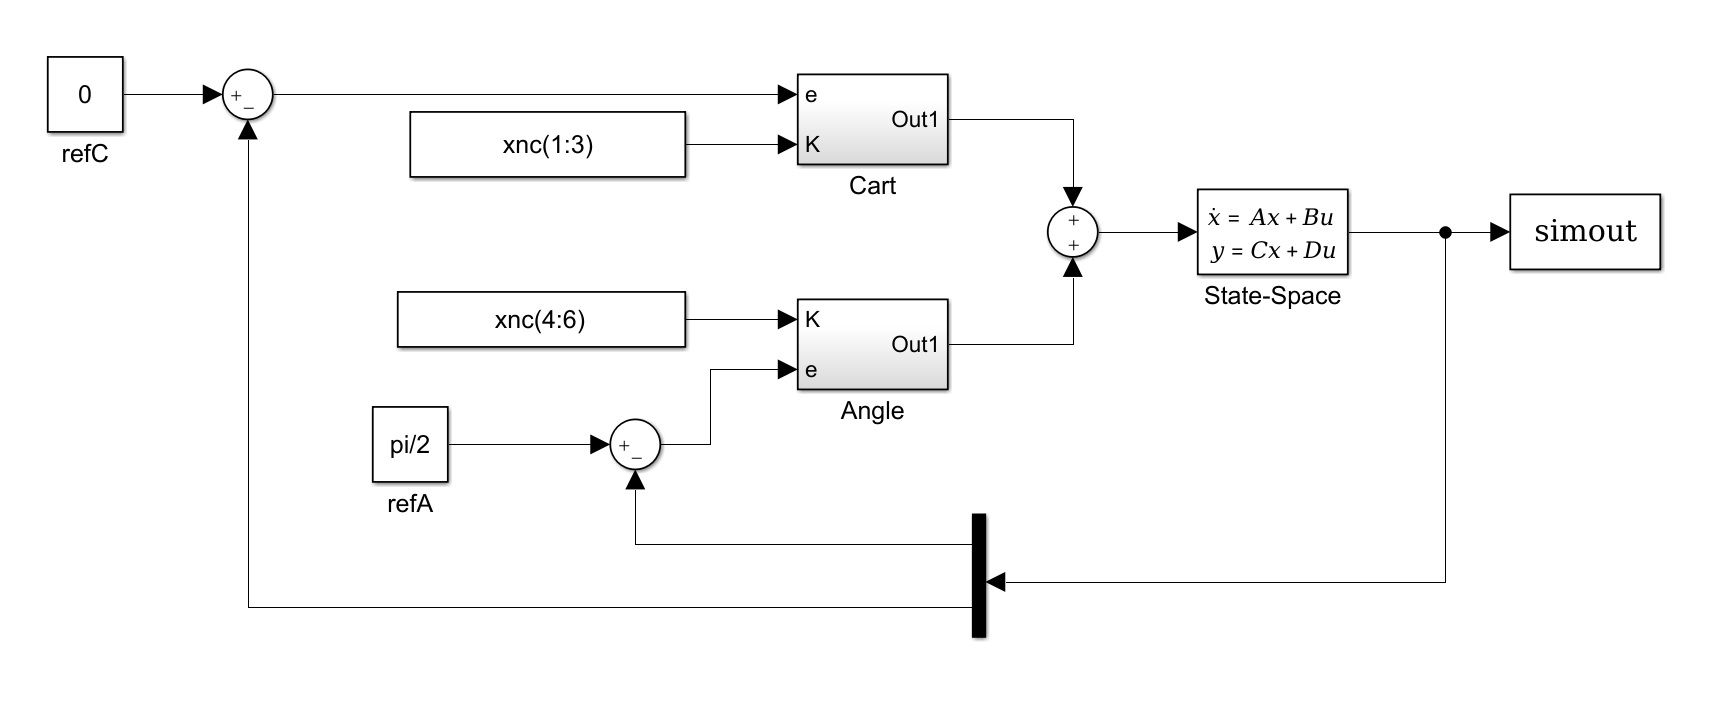
\includegraphics[scale=0.2]{Figuras/control-modelo.jpg}
  \caption{Diagrama de bloques de la implementacion del control PID acoplado} 
\end{figure}

\subsubsection{Estimación de parámetros}
Al momento de diseñar el controlador la parte más compleja es, precisamente, encontrar los
valores óptimos para las constantes $K_i$. Esto se debe principalmente al acoplamiento que
presentan ambos sistemas, pues aunque los controladores se encuentren independientes, ambos
realimentan el mismo sistema, haciendo que los cambios de una variable de estado
inminentemente afecten a la otra. Además, sumado al desconocimiento del efecto que posee cada
párametro sobre el sistema, se hace poco factible una sintonización manual o en métodos estándares. Por lo tanto se opta por plantear la estimación de parámetros
como un problema de optimización no lineal, que busca disminuir el error del estado
estacionario.
Para resolver este problema de optimización se utiliza el método metaheurístico GRASP, el cual es ampliamente aplicado para resolver problemas de optimización combinatoria.
\subsubsection{GRASP}
El método GRASP fue introducido inicialmente por~\cite{Feo1989}, con el fin de solucionar
heurísticamente el problema del conjunto cobertura, un importante problema NP-completo.
Sin embargo, con el tiempo fue adaptado para resolver diferentes problemas.
El algoritmo parte de una solución inicial (en este caso un conjunto de constantes $K_i$
aleatorias e iterativamente realiza modificaciones sobre dicha soluciones, que se realiza
alternando las diferentes constantes de manera independiente a la misma solución y luego se
evalúa cada uno de los nuevos conjuntos de parámetros en la función objetivo. En un algoritmo
voraz clásico se escogería como la siguiente solución el mejor movimiento que mejore la solución
anterior; sin embargo, con esta manera de proceder se puede caer muy fácilmente en un óptimo local. El método
GRASP plantea una manera diferente de proceder considerando las $n$ mejores soluciones y de éstas
considera una aleatoria, aumentando así la diversidad en las soluciones y haciendo más complicado caer en
en óptimo local.\\

La mejor solución encontrada por el método fue
\[K = [-0.5156,\   -3.5156,\   -1.0000,\    3.5156,\         0,\    1.5156]\]

y la respuesta al impulso puede verse en la figura~\ref{fig:controlS}
\begin{figure}[t]
  \label{fig:controlS}
  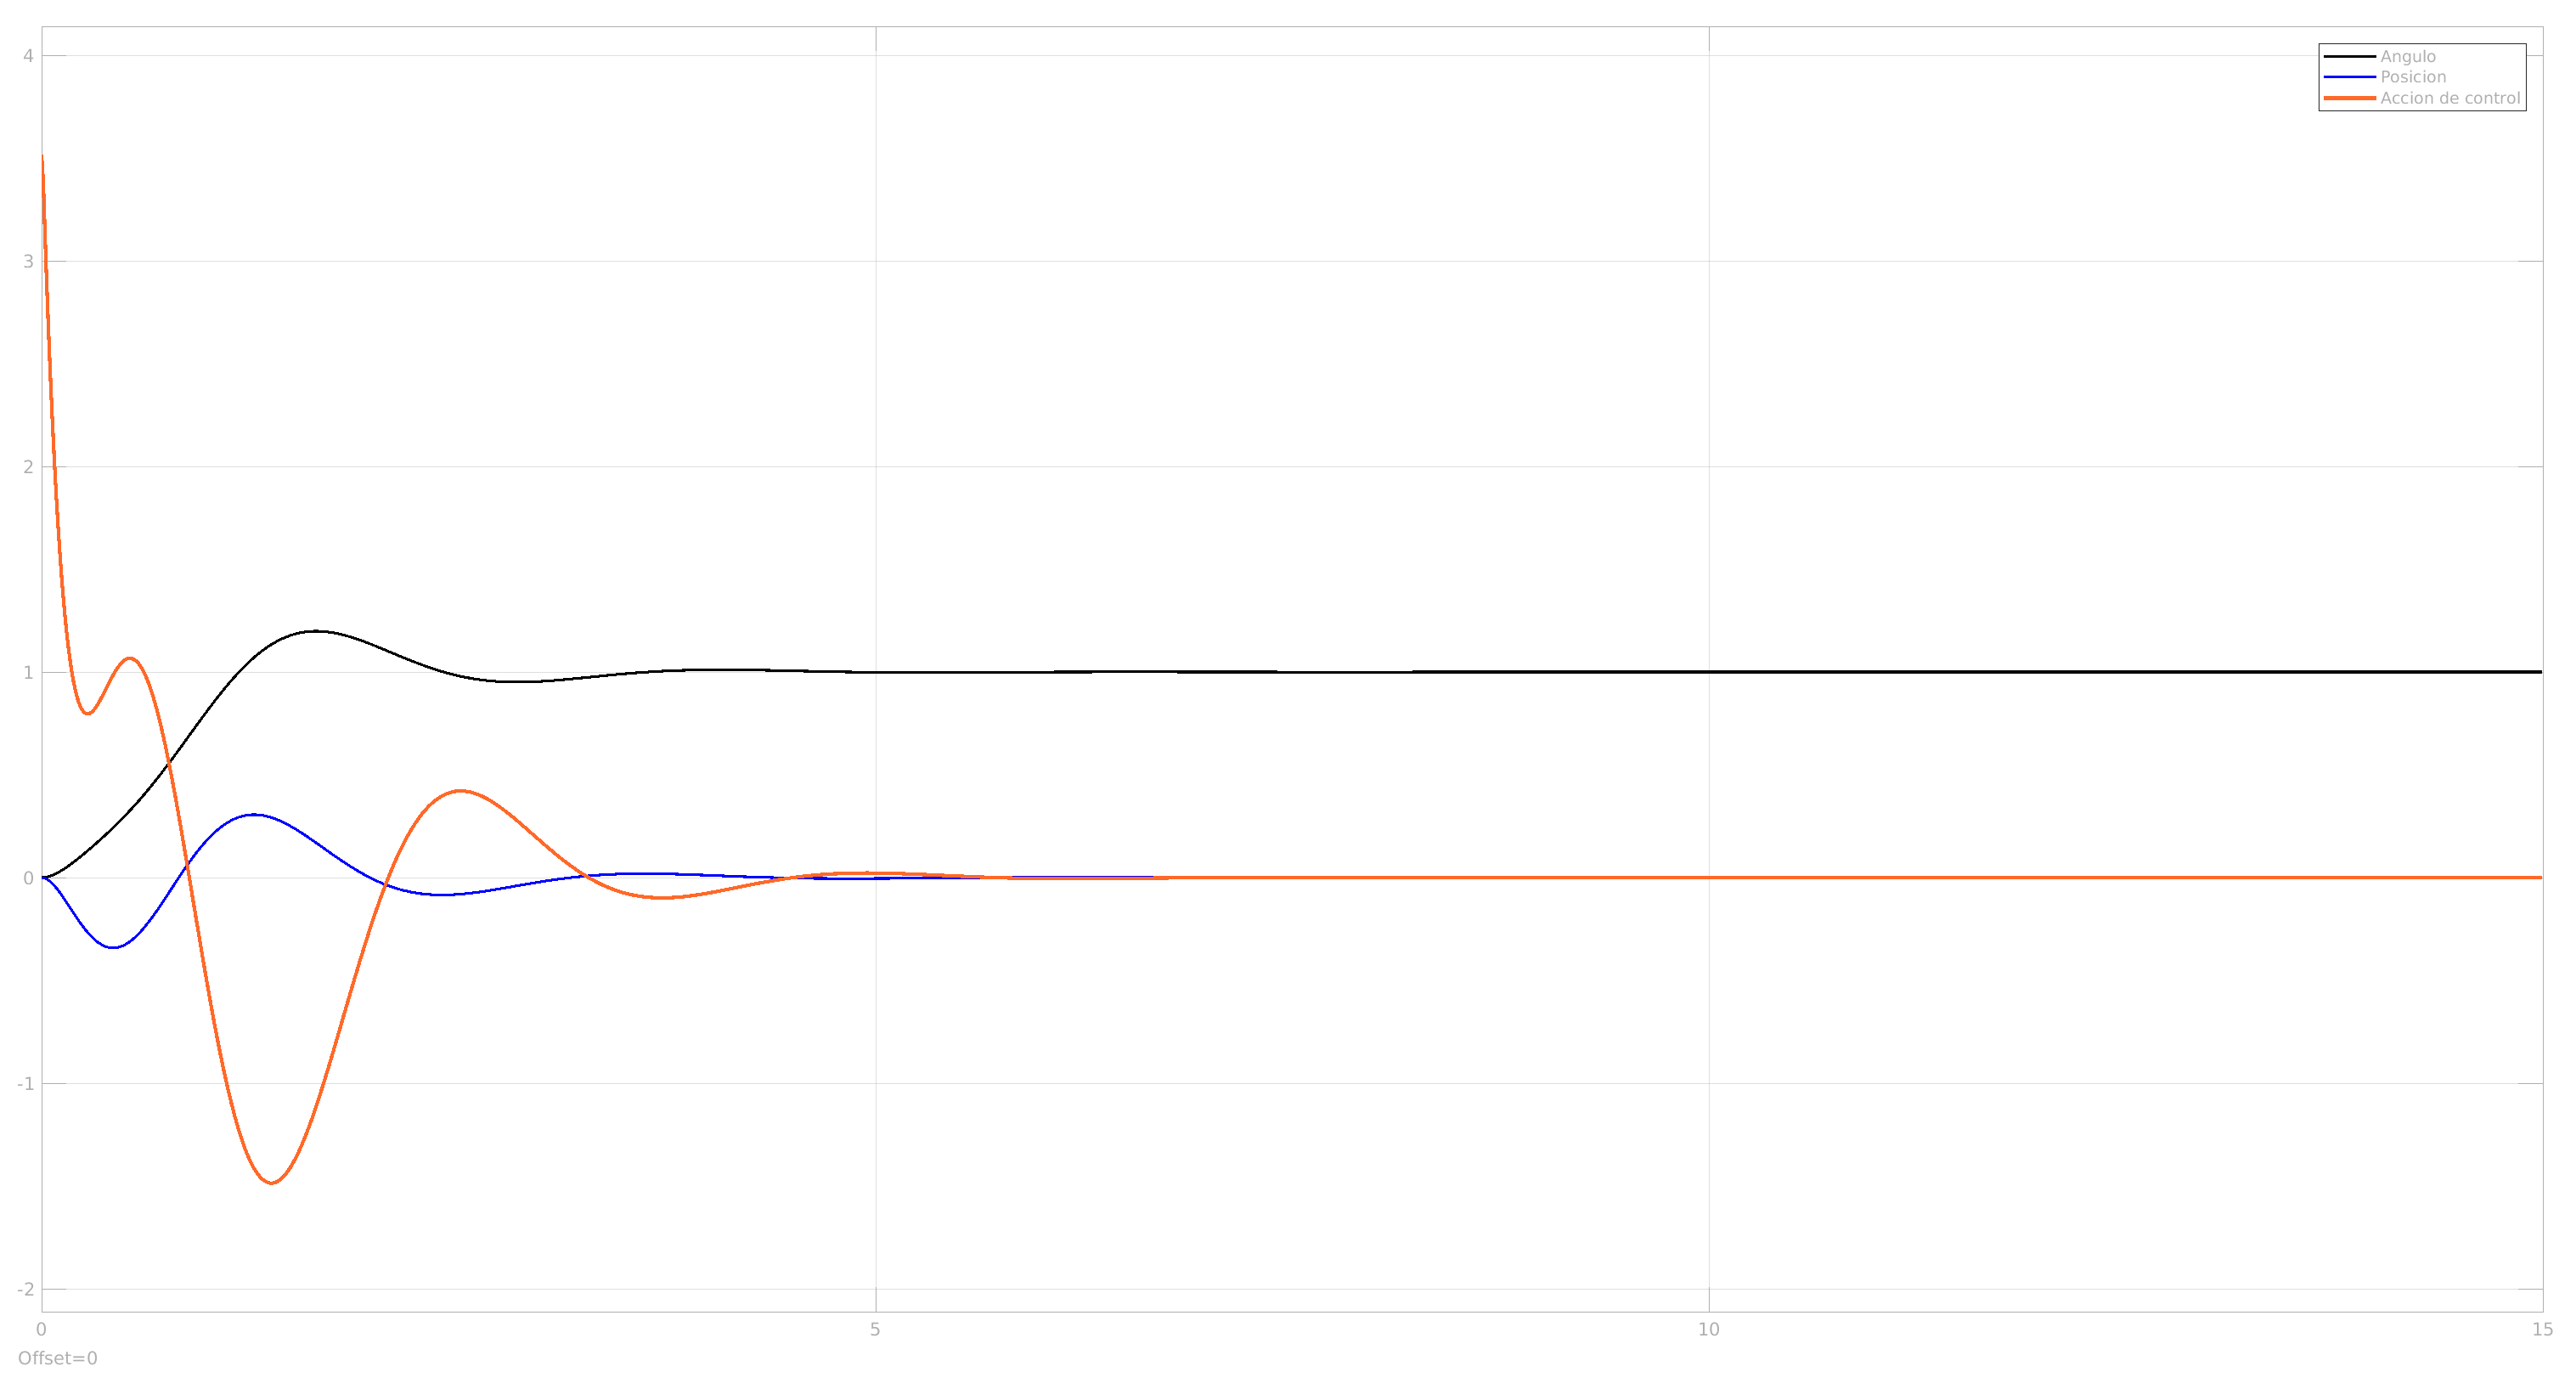
\includegraphics[scale=0.15]{Figuras/controlS}
  \caption{Diagrama de bloques de la implementacion del control PID acoplado} 
\end{figure}

Con base en la respuesta anterior puede verse que el control es capaz de controlar apropiadamente ambas
señales a su señal de referencia, lo cual puede llegar a ser una gran ventaja en comparación
a lo controladores presentados anteriormente. Adicionalmente, al plantear la sintonización del
controlador como un problema de optimización, es posible resolverlo con diferentes métodos, tales
como algoritmos genéticos, los cuales en principio permitirían tener un control inteligente.
